\chapter{Results}\label{chap:Results}

\section{Performance of NLopt}

To test the performance of NLopt, a nonlinear optimization library, trajectories of different length were optimized. Figure \ref{pic:differentGoal} depicts a start vertex and 6 different goal vertices.The figure is in bird's eye perspective and shows a crossing of different hallways. The blue cells represents the floor and the green cells represents the walls. The map was generated with a stereo camera and was not reworked. Therefore some of the cells of the floor which should be occupied/blue are left free. In some of the hallways, there are objects blocking (part of) the way. This passages are tagged with "Bottleneck". Please note that other passages which may look like a bottleneck, such as the top right corner, are not blocked. The green boxes in this passage are part of the ceiling.

\begin{figure}[h]
   \centering
   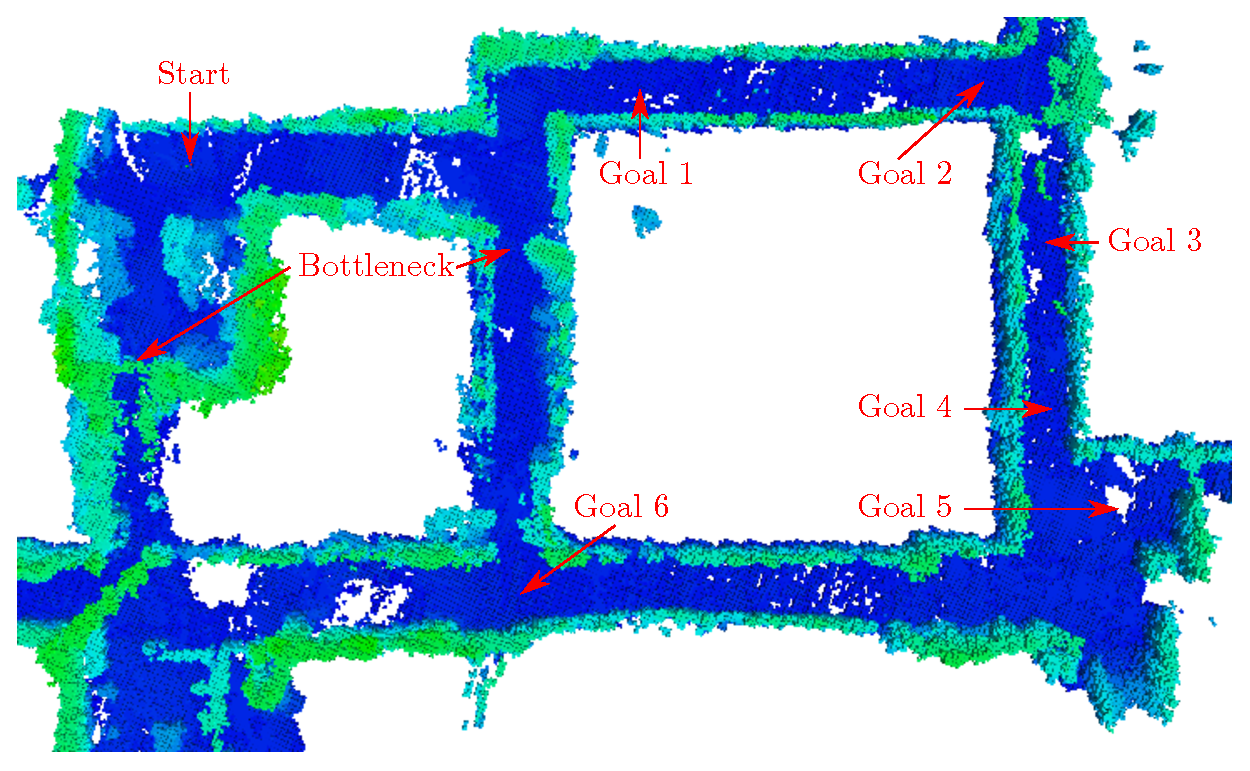
\includegraphics[width=1\textwidth]{pics/ML4.eps}
   \caption{Ein Bild.}
   \label{pic:differentGoal}
\end{figure}

%\begin{figure}[h]
%   \centering
%   \includegraphics[width=0.5\textwidth]{pics/MapLine.png}
%   \caption{Ein Bild.}
%\end{figure}
%
%
%\begin{figure}[h]
%   \centering
%   \includegraphics[width=0.5\textwidth]{pics/MapPoly.png}
%   \caption{Ein Bild.}
%\end{figure}

The bottleneck in the center of figure \ref{pic:differentGoal} gets significant for large bounding boxes. If the dimension of the bounding box are larger than $0.5m$ x $0.5m$ x $0.5m$ the trajectory is not able to pass the bottleneck. Hence, a trajectory with a large bounding box has to go all the way around to proceed from the start vertex to "Goal 6" as depicted in figure \ref{pic:Goal6}.


\begin{figure}[ht]
   \centering
   \includegraphics[angle=90, width=1\textwidth]{pics/MapNlopt.png}
   \caption{Ein Bild.}
   \label{pic:Goal6}
\end{figure}

blablabla


%
%\begin{figure}
%\centering
%\begin{subfigure}{.5\textwidth}
%  \centering
%  \includegraphics[width=1\linewidth]{pics/MapPoly.png}
%  \caption{A subfigure}
%  \label{fig:sub1}
%\end{subfigure}%
%\begin{subfigure}{.5\textwidth}
%  \centering
%  \includegraphics[width=1\linewidth]{pics/MapNlopt.png}
%  \caption{A subfigure}
%  \label{fig:sub2}
%\end{subfigure}
%\caption{A figure with two subfigures}
%\label{fig:test}
%\end{figure}

